%\documentclass[twocolumn,aps]{revtex4-2}


\documentclass[aps,prb,twocolumn,superscriptaddress]{revtex4}

\usepackage{graphicx}
\usepackage{amsmath}

\begin{document}
\title{Quasicrystals and Prime Numbers}

\author{Michael Shaughnessy}
\email{mickeyshaughnessy@gmail.com}
\author{CY Fong}
\email{fong@solid.physics.ucdavis.edu}

\begin{abstract}
This section is the abstract. We describe a pair of transformations (exponential and Fourier) of the distribution of prime numbers. We establish a few properties of the distribution of primes as it relates to scattering. We calculate the scattering amplitude function as a volume in the space of amplituhedrons  
\end{abstract}

\maketitle

\section{Introduction}
Consider a scattering potential and it's Fourier transform:
\begin{equation}
 \label{eq: RiemannFourier}
 \mathcal{F}\left \{ \sum_{\gamma_n \in X}\delta_D(\gamma - \gamma_n) \right \} = \sum_{k_m \in X^{*}} F_{m} \delta_D(k - k_{m}),
\end{equation}


According to Dyson's quasicrystal hypothesis, if we can show the distribution of the prime numbers (2, 3, 5, 7, 11, 13, 17, 19, 23, 29,...) has a quasicrystalline structure, meaning the scattering spectrum of the distribution is a Cantor set of zero measure (point-like), then we can identify the 1-dimensional quasicrystal whose corresponding spectrum is the zeros of the famed Riemann Zeta Function (RZF). 

The prime numbers present a special challenge for discussions of scattering, because scattering, and the associated spectral patterns, is understood with the mathematical tool of the Fourier transform, which allows to change variables between real-space coordinates $(x)$ and the coordinates of reciprocal momentum space representation, $(k)$. We suggest first applying a 1-dimensional change of variables from $x$ to $\frac{1}{\ln{x}}$. 



The boundaries of the amplituhedron, $A$, are where the volume form logarithmically diverges, so in computing scattering amplitudes, it's natural to consider such a logarithmic change of variables. 

\begin{align}
x \rightarrow \frac{x}{\ln(x)}
\end{align}

before applying the Fourier transform 

\begin{equation}
F(k) = \int_{-\infty}^{\infty}f(x)\exp^{2\pi ikx}dx
\end{equation}

In terms of the 



For certain spiral distributions \cite{Varma2016}, related to the Fibonacci sequence, it has been shown that the spectrum may be a Cantor set of measure zero.

%What is the spectrum of the transformed prime numbers? Is it a Cantor set of zero measure?


%\begin{equation}
%\sum_{\gamma_n \in X}\delta_D(\gamma - \gamma_n) 
%\end{equation}

\begin{figure}[h]
  \centering
  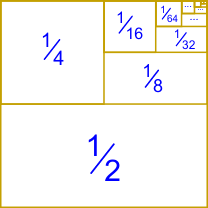
\includegraphics[width=0.5\columnwidth]{square_fractions.png}
  \caption{The sum of $\frac{1}{2} + \frac{1}{4} + \frac{1}{8} + \ldots$}
\end{figure}

\begin{figure}[h]
  \centering
    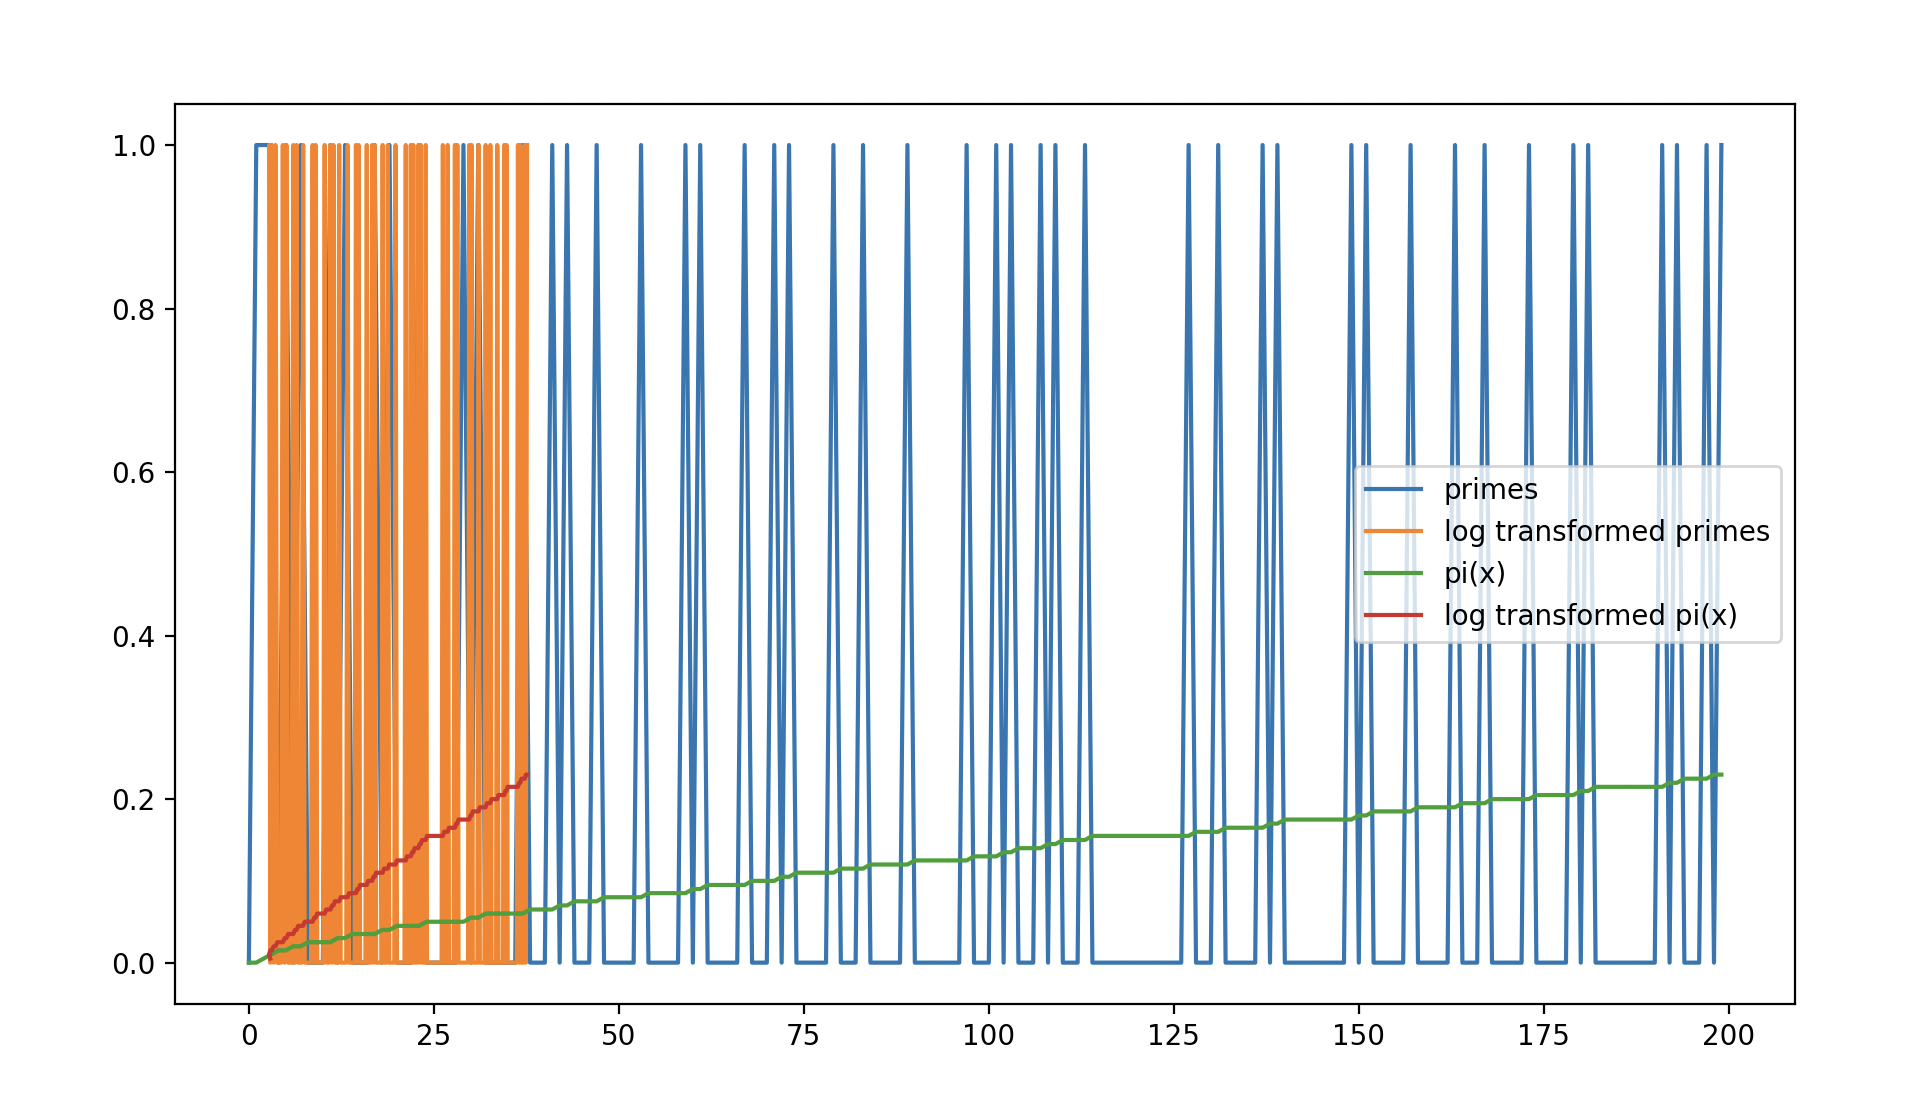
\includegraphics[width=0.5\columnwidth]
  {primes.png}
    \caption{The prime and exponentially squished prime scattering potentials and associated prime counting functions}
\end{figure}

\begin{figure}[h]
  \centering
    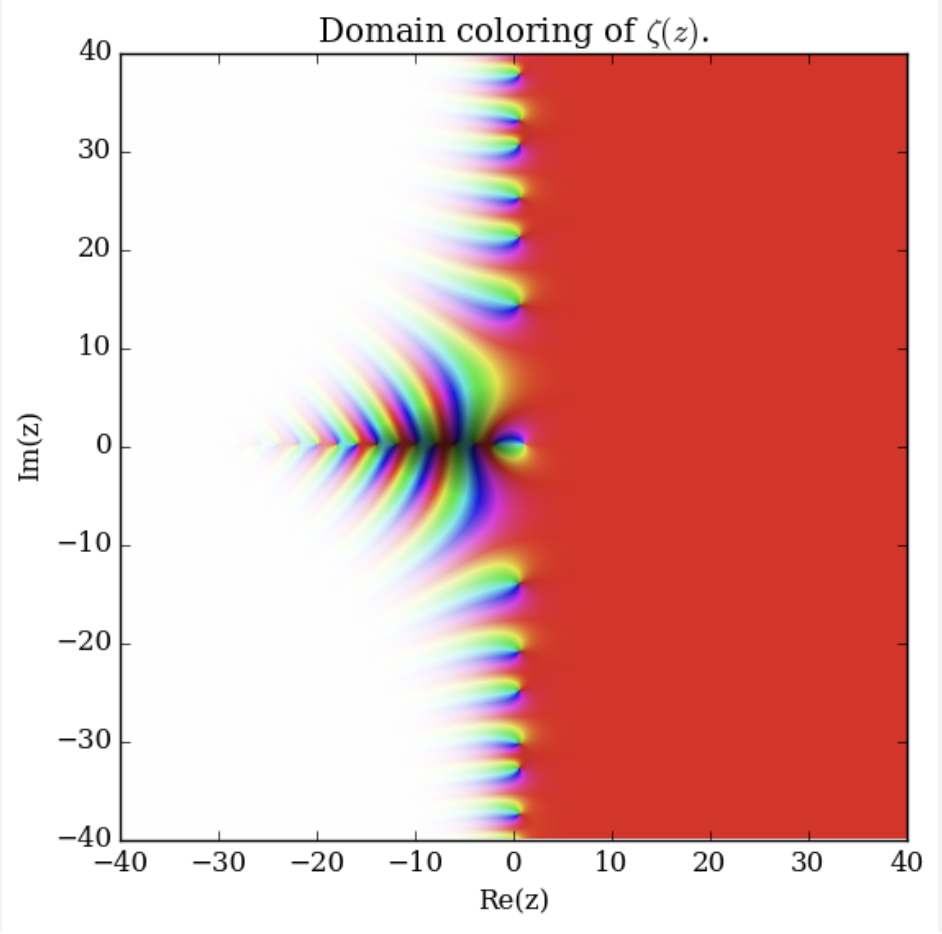
\includegraphics[width=0.5\columnwidth]
  {RZF.png}
    \caption{The zeros of the Riemann zeta function are the tips of the feathers extending in the vertical direction.}
\end{figure}

\begin{figure}[h]
  \centering
    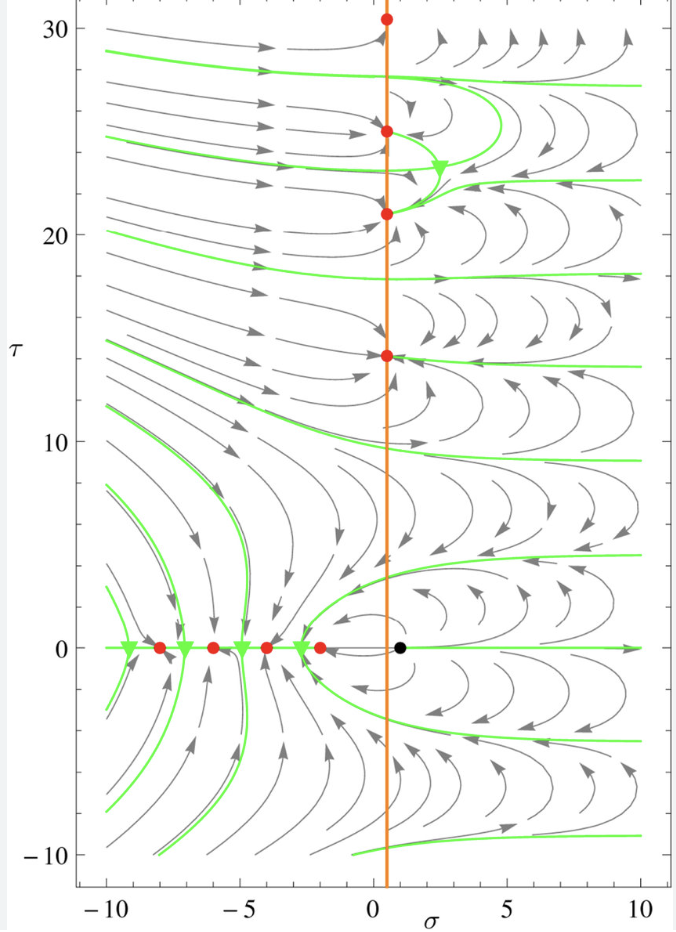
\includegraphics[width=0.5\columnwidth]
  {vector_flow.png}
    \caption{Newton flow vector representation of the RZF}
\end{figure}


\section{Amplituhedron}
   Instead of considering triangulations as in \cite{ArakaniHamed_2014}, we consider decompositions into hyper-rectangular volumes as the basic building block of scattering amplitudes. In this concept  it's natural to consider primes   


\section{Conclusion}

This is the conclusion of the document.

\end{document}




This is a short paper on the quasicrystalline distribution of the prime numbers and the associated scattering properties of physical Al-Mn quasicrystals

